\documentclass{article}
\usepackage[UTF8]{ctex}
\usepackage{float}
\usepackage{graphicx}

\title{二叉树和节点的逻辑设计}
\author{林敬翊}
\date{2022年11月2日}

\begin{document}

\maketitle

\section{设计思路}
    开始时 无论我们提到什么树,我们都需要TreeNode。TreeNode具有标识作用。所以我们在private里声明左指针和右指针,并且具有获取元素,另指针赋值等元素。
    \\
    \\
    BinaryTree 中我们采用的是基出的TreeNode,然后里面具有判断他是否在树中、插入数值、打印、判断树、以及删除功能等等。
    \\
    \\
    BinarySearchTree里我们包含了BinaryTree类,所以继承了所有BinaryTree里的所有函数,然后也新增了一个clone指针的指针等等。然后BinarySearchTreeNode也是应用了TreeNode。
    \\
    \\
    AvlTree里我们里一样包含了BinaryTree类,但是他新增了Balance的函数,同时还有各种case的旋转情况。此外他的AvlTreeNode里大多数应用了TreeNode,但是最主要的是他多了一个Int height。
    \\
    \\
    SplayTree里我们一样包含了BinaryTree类,但是新增了splay函树。然后SplayTreeNode也是引用了TreeNode里面一样的class。

\begin{figure}[H]
    \centering
    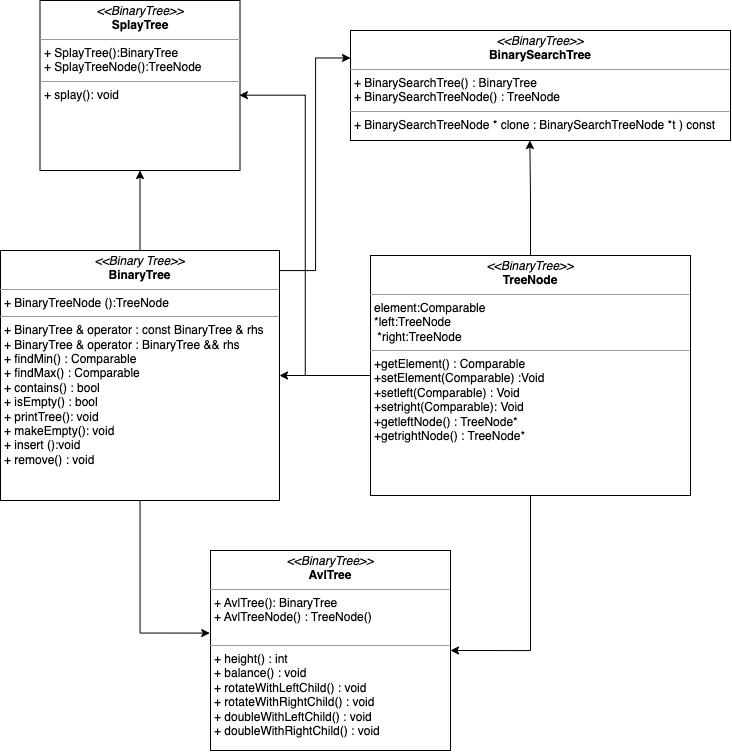
\includegraphics[scale=0.25]{BinaryTree.png}
    \caption{UML 图}
    \label{fig:1}
\end{figure}
    
    

\end{document}
